% ------------------------------------------------------------------------------------------------------------------------------------------------
\chapter{Practical examples of distributed media analysis}
\label{chap:analysis-examples}

This chapter aims to provide tangible examples of how the previously described system preformed and what kind of information was extracted from the reference database when trying to match against disorted media inputs.

The following two sections will focus on practical examples of potential ''attacks'' (disortions) applied to the input media data, and how the proposed system has handled it. The examples have been selected to highlight the two major problems the system has to handle -- distorted image data and time shifted data.

In Section \ref{sec:mirrored-video-detection} video material will be analysed in order to find it's corresponding ''mirrored'' counter-part. This example will also be used to highlight the tremendous possibilities that lie within data \textit{pre-processing} that are applied within the proposed system, and if needed could be expanded even more in order to speed up the system's initial response time.

In Section \ref{sec:scene-detection} an extracted scene will be positioned within an existing video in the reference database. This problem turns out to be non-trivial because of different frame-rates of supplied material, thus search methods similar, in concept, to sub-string search could not have been applied efficiently. The section explains the algorithms applied instead, and showcases an example case.

As this thesis is not focused on development of image analysis algorithms, these sections will instead lean their focus towards the distributed system and big-data parts of the problem. The image comparision algorithms also assume that that the used image correlation algorithm (\textit{phash} -- see Section \ref{sec:phash}) performs well enough for the job at hand. 

\textit{The frames used to illustrate the experiments originate from the movie ''\textit{Big Buck Bunny}'' \cite{big-buck-bunny} which has been created by the Blender Foundation \cite{blender-foundation} and released under the Creative Commons license \cite{creative-commons}.}

% ------------------------------------------------------------------------------------------------------------------------------------------------
\section{Mirrored video detection}
\label{sec:mirrored-video-detection}
In order to test the system in scenarios of image disortion the example case of ''mirrored'' video material was used. This case is fairly popular among material uploaded to YouTube, so outside of the ease of preparing test data, it is also a valid real-life scenario of one might encounter.

\begin{figure}
        \centering
        \begin{subfigure}[b]{0.45\textwidth}
                
\includegraphics[width=\textwidth]{img/Big_Buck_Bunny_normal.png}
                \caption{Original frame}
                \label{fig:original-frame}
        \end{subfigure}
        \begin{subfigure}[b]{0.45\textwidth}
                
\includegraphics[width=\textwidth]{img/Big_Buck_Bunny_mirror.png}
                \caption{Mirrored frame}
                \label{fig:mirrored-frame}
        \end{subfigure}
        \caption{Example of original and mirrored frame}\label{fig:frames-mirrored}
\end{figure}


\subsection{Detecting other kinds of distorions in video material}

Of course, other kinds of disortions could be applied to a video, such as comparing a high-quality video with a low-quality counterpart or simple coloring filters. While being outside of the scope of this thesis, the basic concepts and framework proposed would easily be able to incorporate more scoring functions into the Map Reduce pipeline that would help determine matches between even such disorted video materials. 

An interesting example disortion found commonly in many materials is slight changes in the color hue or white balance of the \todo{histograms}


% ------------------------------------------------------------------------------------------------------------------------------------------------
\section{Scene detection}
\label{sec:scene-detection}
This scenario can be explained as trying to find out \textit{where} (if at all) a scene takes place in a movie known to the reference database. 

Although on the sufrace the general problem statement is not so different than substring search, which is a known and well researched topic in computer science. In sub-string search algorithms like the Knuth–Morris–Pratt \cite{kmp-string-search} or the Boyer-Moore \cite{boyer-string-search} algorithms leverage that the ''matching'' either will apply, or will not in order to increase search speed in the worst case to still linear time. However, these methods can \textit{not} be directly applied to the problem specified in this section -- because of the dissortions in source and reference video material as well as the possibility of cross-matches when a movie is built up from multiple short scenes from other movies -- a typical example here would be ''flash-back'' scenes or ''top 10'' movies where before the last top-3, the movie would quickly go over already shown frames of scenes. Another problem adding to the dissortions is frame rates of reference data vs. an analysed video fragment -- even a slight missmatch (30FPS vs. 25FPS) would render the substring search algorithms not usable for this concrete example.

\begin{figure}[ch!]
  \centering
  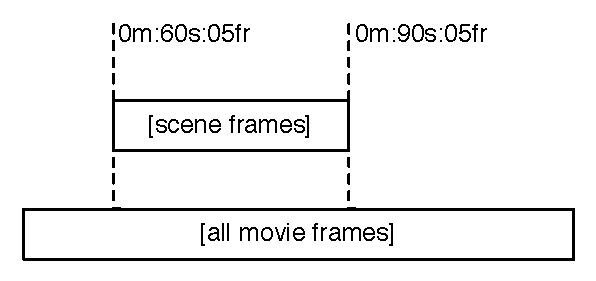
\includegraphics[width=0.6\textwidth]{img/frames-timeline-matching}
  \caption{Visual representation of the goal of this example application.}
\end{figure}

Instead, a more statistical aproach was taken. In which a frame is compared with it's set of ''potential match candidates'' which are determined by very coarse filtering of the reference data set by bucketing certain criteria of their histograms such as ''dominating red'' or ''dominating blue'' (this classification is prepared on the reference data beforehand -- during importing into the system).

\todo{mention somewhere before that we really extract data like ''mostly red''}

\todo{finish this scenario}

\begin{figure}[ch!]
  \centering
  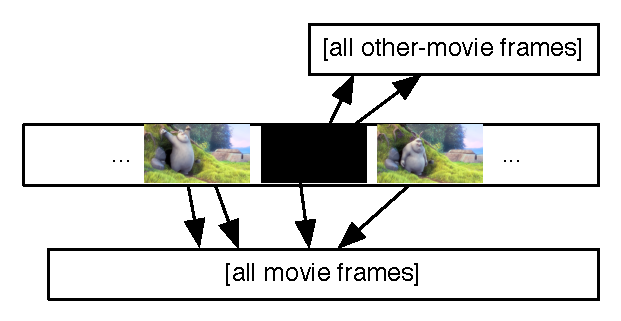
\includegraphics[width=0.6\textwidth]{img/frames-timeline-matching-missmatch}
  \caption{One frame may potentially match multiple reference frames. The final most probable matching scene is determined by aggregating data the direct frame-to-frame matches.}
\end{figure}

